%%%%%%%%%%%%%%%%%%%%%%%%%%%%%%%%%%%%%%%%%
% Beamer Presentation
% LaTeX Template
% Version 1.0 (10/11/12)
%
% This template has been downloaded from:
% http://www.LaTeXTemplates.com
%
% License:
% CC BY-NC-SA 3.0 (http://creativecommons.org/licenses/by-nc-sa/3.0/)
%
%%%%%%%%%%%%%%%%%%%%%%%%%%%%%%%%%%%%%%%%%

%----------------------------------------------------------------------------------------
%	PACKAGES AND THEMES
%----------------------------------------------------------------------------------------

\documentclass{beamer}
\usepackage[utf8x]{inputenc}
\usepackage[T1]{fontenc}
\usepackage{listings}
\usepackage{xcolor}
\usepackage{longtable}
\colorlet{punct}{red!60!black}
\definecolor{background}{HTML}{EEEEEE}
\definecolor{delim}{RGB}{20,105,176}
\colorlet{numb}{magenta!60!black}
\PassOptionsToPackage{hyphens}{url}\usepackage{hyperref}
\hypersetup{
    pdfnewwindow=true,      % links in new window
    colorlinks=true,       % false: boxed links; true: colored links
    %urlcolor=[rgb]{0.45, 0, 0}           % color of external links
}
\definecolor{dkgreen}{rgb}{0,0.6,0}
\definecolor{gray}{rgb}{0.5,0.5,0.5}
\definecolor{light-gray}{gray}{0.95}
\definecolor{mauve}{rgb}{0.58,0,0.82}
\lstset{
    basicstyle=\tiny\ttfamily,
    numbers=left,
    numberstyle=\scriptsize,
    stepnumber=1,
    numbersep=8pt,
    showstringspaces=false,
    breaklines=true,
}
\lstdefinelanguage{json}{
    basicstyle=\normalfont\ttfamily,
    numbers=left,
    numberstyle=\scriptsize,
    stepnumber=1,
    numbersep=8pt,
    showstringspaces=false,
    breaklines=true,
    %frame=lines,
    %backgroundcolor=\color{background},
    literate=
     *{0}{{{\color{numb}0}}}{1}
      {1}{{{\color{numb}1}}}{1}
      {2}{{{\color{numb}2}}}{1}
      {3}{{{\color{numb}3}}}{1}
      {4}{{{\color{numb}4}}}{1}
      {5}{{{\color{numb}5}}}{1}
      {6}{{{\color{numb}6}}}{1}
      {7}{{{\color{numb}7}}}{1}
      {8}{{{\color{numb}8}}}{1}
      {9}{{{\color{numb}9}}}{1}
      {:}{{{\color{punct}{:}}}}{1}
      {,}{{{\color{punct}{,}}}}{1}
      {\{}{{{\color{delim}{\{}}}}{1}
      {\}}{{{\color{delim}{\}}}}}{1}
      {[}{{{\color{delim}{[}}}}{1}
      {]}{{{\color{delim}{]}}}}{1},
}

\mode<presentation> {

% The Beamer class comes with a number of default slide themes
% which change the colors and layouts of slides. Below this is a list
% of all the themes, uncomment each in turn to see what they look like.

%\usetheme{default}
%\usetheme{AnnArbor}
%\usetheme{Antibes}
%\usetheme{Bergen}
%\usetheme{Berkeley}
%\usetheme{Berlin}
%\usetheme{Boadilla}
\usetheme{CambridgeUS}
%\usetheme{Copenhagen}
%\usetheme{Darmstadt}
%\usetheme{Dresden}
%\usetheme{Frankfurt}
%\usetheme{Goettingen}
%\usetheme{Hannover}
%\usetheme{Ilmenau}
%\usetheme{JuanLesPins}
%\usetheme{Luebeck}
%\usetheme{Madrid}
%\usetheme{Malmoe}
%\usetheme{Marburg}
%\usetheme{Montpellier}
%\usetheme{PaloAlto}
%\usetheme{Pittsburgh}
%\usetheme{Rochester}
%\usetheme{Singapore}
%\usetheme{Szeged}
%\usetheme{Warsaw}

% As well as themes, the Beamer class has a number of color themes
% for any slide theme. Uncomment each of these in turn to see how it
% changes the colors of your current slide theme.

%\usecolortheme{albatross}
%\usecolortheme{beaver}
%\usecolortheme{beetle}
%\usecolortheme{crane}
%\usecolortheme{dolphin}
%\usecolortheme{dove}
%\usecolortheme{fly}
%\usecolortheme{lily}
%\usecolortheme{orchid}
%\usecolortheme{rose}
%\usecolortheme{seagull}
%\usecolortheme{seahorse}
%\usecolortheme{whale}
%\usecolortheme{wolverine}

%\setbeamertemplate{footline} % To remove the footer line in all slides uncomment this line
%\setbeamertemplate{footline}[page number] % To replace the footer line in all slides with a simple slide count uncomment this line

%\setbeamertemplate{navigation symbols}{} % To remove the navigation symbols from the bottom of all slides uncomment this line
}

\usepackage{graphicx} % Allows including images
\usepackage{booktabs} % Allows the use of \toprule, \midrule and \bottomrule in tables
\usepackage{amssymb}  % Allows symbols

\usepackage{color}
\usepackage{subfigure}

\renewcommand\footnotemark{}
\renewcommand\footnoterule{}

%----------------------------------------------------------------------------------------
%	TITLE PAGE
%----------------------------------------------------------------------------------------

\title[LiES]{LiES - Linear Equations Systems Solver} % The short title appears at the bottom of every slide, the full title is only on the title page
% (Correct use of condoms and SSL) % make subtitle
\subtitle{Sistemi con vincoli}

%\author[Sebastiano Gottardo]{Sebastiano Gottardo} % Your name

\institute[UNIPD] % Your institution as it will appear on the bottom of every slide, may be shorthand to save space
{
\vspace{-1cm}
\begin{figure}

\includegraphics[scale=.3]{common-images/unipd_logo.pdf}\\
\end{figure}
Universita' degli Studi di Padova\\[5mm] % Your institution for the title page
{\large Sebastiano Gottardo\\
Marco Ziccardi\\}
}
\footnotesize{\date{\today}} % Date, can be changed to a custom date

\begin{document}

\begin{frame}
\titlepage % Print the title page as the first slide
\end{frame}

\begin{frame}
\frametitle{Indice} % Table of contents slide, comment this block out to remove it

\tableofcontents % Throughout your presentation, if you choose to use \section{} and \subsection{} commands, these will automatically be printed on this slide as an overview of your presentation

\end{frame}

%----------------------------------------------------------------------------------------
%	PRESENTATION SLIDES
%----------------------------------------------------------------------------------------

\section{Introduzione}

\begin{frame}
\frametitle{LiES}
\begin{block}{}
LiES (Linear Equations Solver) è un risolutore di sistemi di equazioni lineari
\end{block}

Offre diverse funzionalità su sistemi di equazioni lineari:

\begin{itemize}
	\item Generazione 
	\item Salvataggio su file
	\item Caricamento da file
	\item Risoluzione, con diverse strategie
		\begin{itemize}
			\item Backtrack
			\item Bactrack, con variabile più vincolata
			\item Backtrack, con consistenza sugli archi
			\item Branch and bound
			\item Branch and bound, con consistenza sugli archi
		\end{itemize}
\end{itemize}
%
%\begin{figure}
%\centering
%	\includegraphics[scale=0.3]{images/mithys/table}
%\end{figure}
%
%\begin{itemize}
%	\item Fully consistent with Fahl et al.'s results
%	\item Twitter and Voxie are the only two PenProof applications
%\end{itemize}
%
\end{frame}

\section{Generazione di CSP}

\begin{frame}
\frametitle{Generatore Casuale di CSP}

\begin{itemize}
	\item LiES genera problemi casualmente a partire da:
\begin{center}
	\textit{B(k,n,d,$p_1$,$p_2$)}
\end{center}
	\begin{itemize}
		\item k - arietà dei vincoli
		\item n - numero di variabili
		\item d - grandezza dei domini
		\item $p_1$ - densità del grafo di vincoli
		\item $p_2$ - strettezza dei vincoli
	\end{itemize}
	\item Genera problemi in formato JSON
\end{itemize}

\end{frame}

\begin{frame}[fragile]
\frametitle{Formato di un CSP}
I problemi generati hanno il seguente formato:

\hspace{1cm}~\begin{minipage}[c]{.9\textwidth}
\begin{lstlisting}[language=json]
{
	"vnum": 		m,
	"cnum":			n,
	"coeffs":		[a11, a12, ..., amn],
	"cterms":		[b1, ..., bm],
	"domains":	[[l1, h1], ..., [ln, hn]]
}
\end{lstlisting}
\end{minipage}
\end{frame}

\section{Strategie di risoluzione}


\begin{frame}
\frametitle{Backtrack}

\begin{itemize}
	\item Prima tecnica realizzata: \textit{forward checking} con \textit{backtrack}
	\item Costruisce l'albero di \textit{labeling} ridotto del problema
	\item Dato un ordinamento $x_1, ..., x_n$ delle variabili:
		\begin{itemize}
			\item Discendenti diretti della radice sono della forma $(x_1, d)$
			\item Discendenti diretti di un nodo $(x_j, d)$ per $i \in \left [ 1, n-1 \right ]$ sono della forma $(x_{j+1}, d)$
			\item I suoi rami determinano solo istanziazioni consistenti
		\end{itemize}
	\item Nessuna propagazione di vincoli
\end{itemize}

\end{frame}

\begin{frame}[fragile]
\frametitle{Backtrack - Flusso d'esecuzione}
L'albero di \textit{labeling} è costruito tramite la funzione \texttt{solve\_rec} che opera come segue:
\begin{enumerate}
\item Il dominio della variabile corrente viene salvato
\item Si itera sui valori nel dominio della variabile corrente, l'iterazione termina quando il dominio è vuoto oppure quando in un qualche sotto-albero è stata trovata una soluzione
	\begin{enumerate}
		\item Viene selezionato un assegnamento per la variabile corrente (si seleziona sempre il minimo valore nel dominio)
		\item Si controlla che la soluzione finora ottenuta, seppur parziale, sia consistente
		\item Se l'assegnamento è consistente e la variabile assegnata è l'ultima allora è stata trovata una soluzione
		\item Altrimenti l'assegnamento correntemente esaminato viene annullato
	\end{enumerate}
\item Se nessuna soluzione è stata trovata nell'intero sotto-albero il dominio della variabile corrente viene ripristinato
\end{enumerate}
\end{frame}

\begin{frame}
\frametitle{Backtrack, \textit{most constrained}}

\begin{itemize}
	\item \textit{forward checking} con \textit{backtrack}
	\item Nessuna propagazione di vincoli
	\item Diverso ordine di selezione delle variabili
	\item \textit{most constrained variable heuristic} 
		\begin{itemize}
			\item Si assegna la viariabile non ancora assegnata che compare nel maggior numero di vincoli
		\end{itemize}
	\item Ordinamento ottenuto tramite una pre-elaborazione
\end{itemize}

\end{frame}

\begin{frame}
\frametitle{Backtrack, \textit{arc consistency}}

\begin{itemize}
	\item \textit{forward checking} con \textit{backtrack} e propagazione di vincoli
	\item Criterio di consistenza: \textit{arc consistency}
	\item Utilzza algoritmo \texttt{AC-3}
	\item Ha complessità $O(ek^3)$
		\begin{itemize}
			\item $e$: numero di vincoli del problema
			\item $k$: dimensione dei domini
		\end{itemize}
	\item \textit{Arc consistency} restringe i domini partendo da vincoli binari
		\begin{itemize}
			\item Fase di pre-elaborazione per identificarli tutti
		\end{itemize}
\end{itemize}

\end{frame}

\begin{frame}
\frametitle{\textit{Arc consistency} - Flusso d'esecuzione}

\begin{enumerate}
	\item Creata una collezione con i vincoli binari la cui consistenza sugli archi deve ancora essere controllata
	\item Si itera finchè la suddetta collezione non è vuota
	\begin{enumerate}
		\item Si identificano i domini delle variabili coinvolte, siano esse $x_1$ e $x_2$
		\item Si itera su ciascun possibile valore delle variabili $x_1$ e $x_2$
		\begin{enumerate}
			\item Si controlla che il vincolo selezionato sia consistente sui valori selezionati
			\item Se per nessun valore della variabile $x_2$ il valore della variabile $x_1$ verifica il vincolo tale valore va rimosso dal dominio di $x_1$
		\end{enumerate}
		\item Se il dominio di $x_1$ è cambiato vanno inseriti nella collezione di vincoli da esaminare tutti quelli su una qualsiasi variabile $x_j$ con $j\neq1$ e $x_1$
		\item Il vincolo appena considerato viene eliminato dalla collezione
	\end{enumerate}
\end{enumerate}

\end{frame}

\begin{frame}
\frametitle{Branch and Bound}

\begin{itemize}
	\item Ricerca la soluzione ottima secondo una data funzione obiettivo $f$
	\item Mantiene valore $bound$: il valore della funzione obiettivo per la migliore soluzione finora
	\item Usa funzione euristica $h$ per valutare soluzioni incomplete
	\item Se su un nodo $h$ è peggiore di $bound$:
	\begin{itemize}
		\item Viene escluso dalla ricerca l'intero sotto-albero
	\end{itemize}
	\item Minimazza la funzione:
\begin{equation*}
f(X) = \sum_{i \in [0,n-1]:~i~is~even} x_i
\end{equation*}
	\item Usa l'euristica:
\begin{equation*}
h(X) = \sum_{i \in [0,n-1]:~i~is~even} min(x_i)
\end{equation*}
\end{itemize}

\end{frame}

\begin{frame}
\frametitle{Branch and Bound, \textit{arc consistency}}

\begin{itemize}
	\item Ricerca soluzione ottima come classico \textit{branch and bound}
	\item Minimizza $f$ e utilizza la stessa euristica
	\item Utilizza propagazione di vincoli
	\item Criterio di consistenza: \textit{arc consistency}
	\item Stesso algoritmo della risoluzione \textit{backtrack}
\end{itemize}

\end{frame}

\section{Test}

\begin{frame}[fragile]
\frametitle{Test1}
\hspace{1cm}~\begin{minipage}[c]{.9\textwidth}
\begin{lstlisting}[language=json, basicstyle=\small]
{
	"vnum": 		3,
	"cnum":			3,
	"coeffs":		[1, 0, 1, 1, 0, 1, 0, 1, 0],
	"cterms":		[10, 10, 5],
	"domains":	[[-10, 10], [0, 10], [0, 10]]
}
\end{lstlisting}
\end{minipage}
\begin{minipage}[c]{.35\linewidth}
\begin{footnotesize}
\begin{longtable}{c c c}
\toprule
\textbf{Algorithm} & \textbf{Time (ms)} & \textbf{Nodes}\\
\midrule
\texttt{Backtrack} & 0,515 & 248 \\
\midrule
\texttt{MC\_Backtrack} & 0,295 & 138 \\
\midrule
\texttt{AC\_Backtrack} & 0,075 & 8 \\
\bottomrule
\end{longtable}
\end{footnotesize}
\end{minipage}\hspace{1cm}~
\begin{minipage}[c]{.5\linewidth}
\begin{figure}[!h]
\begin{center}
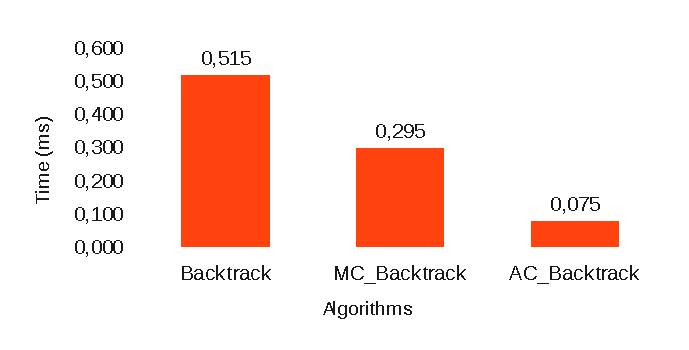
\includegraphics[scale=0.55]{./report-images/test1_time.pdf}
\end{center}
\end{figure}
\end{minipage}
\end{frame}

\begin{frame}[fragile]
\frametitle{Test2 (1)}
\begin{tiny}
\begin{tabular}{c | c | c | c c | c c | c c}
\textbf{Problem} & \textbf{Variables} & \textbf{Status} & \multicolumn{2}{c}{\textbf{Backtrack}} & \multicolumn{2}{c}{\textbf{MC\_Backtrack}} & \multicolumn{2}{c}{\textbf{AC\_Backtrack}} \\
 & & & \textbf{Nodes} & \textbf{Times (ms)} & \textbf{Nodes} & \textbf{Times (ms)} & \textbf{Nodes} & \textbf{Times (ms)}\\
\toprule
cspa.json & SOLVED & 4 & 1267 & 653,435 & 67 & 11,714 & 4 & 3,394 \\
\midrule
cspb.json & FAILED & 5 & 8840 & 8217,945 & 8840 & 9376,913 & 8422 & 7755,468 \\
\midrule
cspc.json & FAILED & 6 & 168420 & 118,939 & 8420 & 6,66 & 0 & 0,025 \\
\midrule
cspe.json & FAILED & 7 & 3368420	& 3443,583 & 8420 & 7,329 & 0 & 1,952 \\
\midrule
cspd.json & FAILED & 8 & 168420 & 263,697 & 420 & 1,877 & 0 & 0,096 \\
\midrule
cspf.json & FAILED & 9 & 3368420	& 2732,075 & 420 & 1,279 & 0 & 0,031 \\
\midrule
cspg.json & FAILED & 10 & 168420	& 161,748 & 8420 & 7,275 & 0 & 0,038 \\
\midrule
csph.json & FAILED & 11 & 3368420 & 6513,557 & 168420 & 155,434 & 0 & 0,035 \\
\midrule
cspi.json & FAILED & 12 & 176820	& 243,419 & 168420 & 228,973 & 0 & 0,036 \\
\bottomrule
\end{tabular}
\end{tiny}
\end{frame}

\begin{frame}[fragile]
\frametitle{Test2 (2)}

\vspace{-.3cm}

\begin{figure}[!h]
\begin{center}
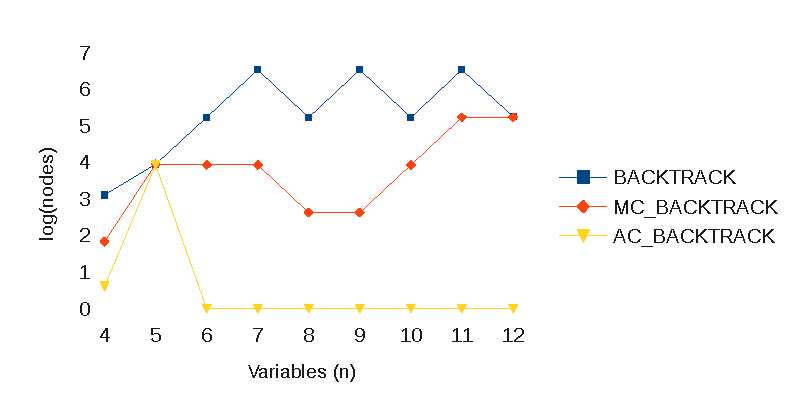
\includegraphics[scale=0.58]{./report-images/test2_nodes.pdf}
\end{center}
\end{figure}

\vspace{-.7cm}

\begin{figure}[!h]
\begin{center}
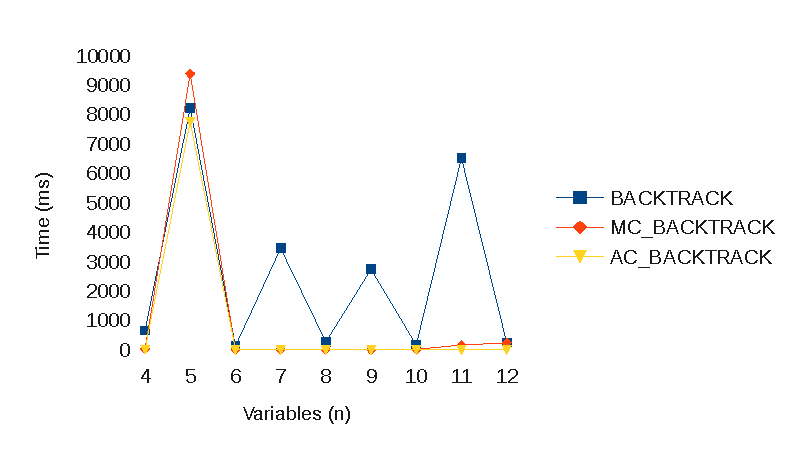
\includegraphics[scale=0.58]{./report-images/test2_time.pdf}
\end{center}
\end{figure}

\end{frame}

\begin{frame}
\frametitle{Test3}

\begin{longtable}{c c c}
\toprule
\textbf{Algorithm} & \textbf{Time (ms)} & \textbf{Nodes}\\
\midrule
\texttt{BB} & 344,155 & 483 \\
\midrule
\texttt{AC\_BB} & 9,926 & 23 \\
\bottomrule
\end{longtable}

\vspace{.5cm}

\begin{minipage}[c]{.4\linewidth}
\begin{figure}[!h]
\begin{center}
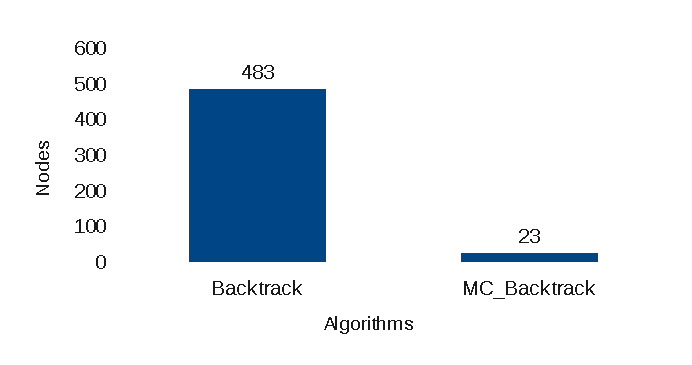
\includegraphics[scale=0.55]{./report-images/test3_nodes.pdf}
\end{center}
\end{figure}
\end{minipage}\hspace{1cm}~
\begin{minipage}[c]{.4\linewidth}
\begin{figure}[!h]
\begin{center}
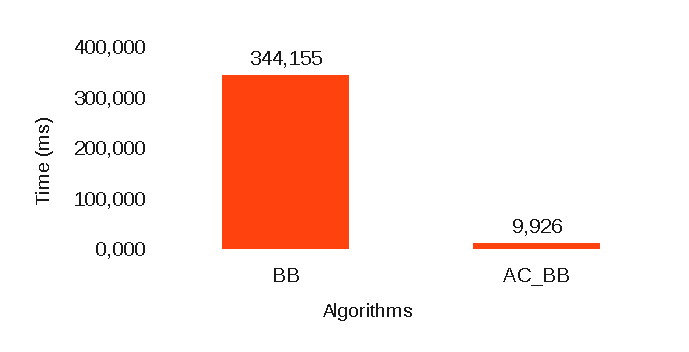
\includegraphics[scale=0.55]{./report-images/test3_time.pdf}
\end{center}
\end{figure}
\end{minipage}

\end{frame}


%----------------------------------------------------------------------------------------

\end{document} 
